\begin{figure}[!p]
    \centering
    \begin{subfigure}[b]{\SideBySidePlotWidth}
        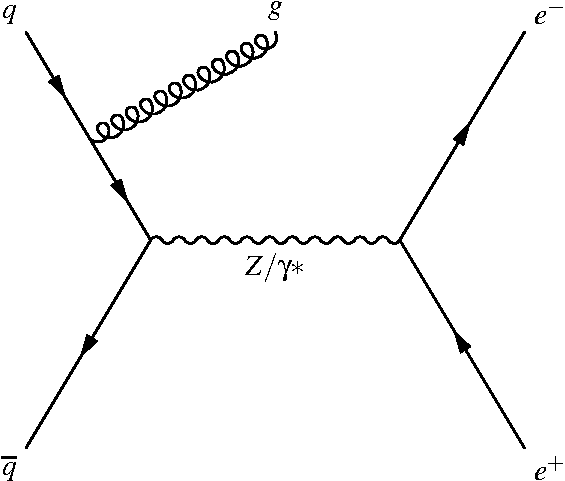
\includegraphics[width=\linewidth]{figures/feyn_qqbar_to_zg.pdf}
        \caption{}
        \label{fig:feyn_qqbar_to_zg}
    \end{subfigure}%
    \begin{subfigure}[b]{\SideBySidePlotWidth}
        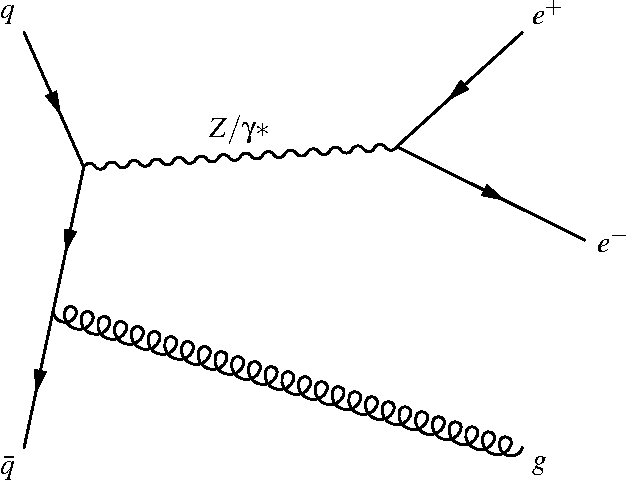
\includegraphics[width=\linewidth]{figures/feyn_qbarq_to_zg.pdf}
        \caption{}
        \label{fig:feyn_qbarq_to_zg}
    \end{subfigure}
    \begin{subfigure}[b]{\SideBySidePlotWidth}
        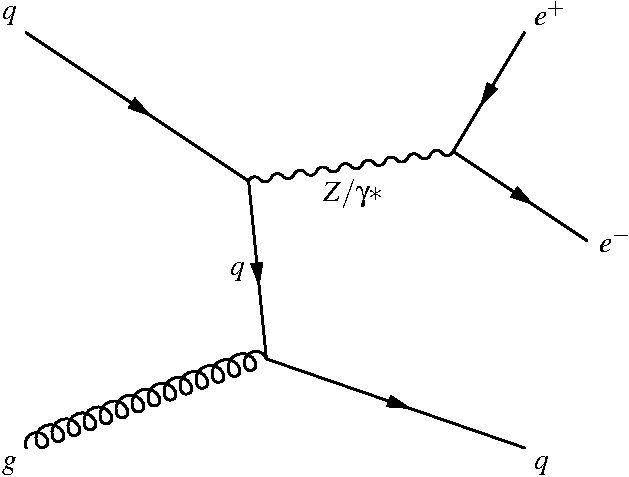
\includegraphics[width=\linewidth]{figures/feyn_qg_to_zq.pdf}
        \caption{}
        \label{fig:feyn_qg_to_zq}
    \end{subfigure}%
    \begin{subfigure}[b]{\SideBySidePlotWidth}
        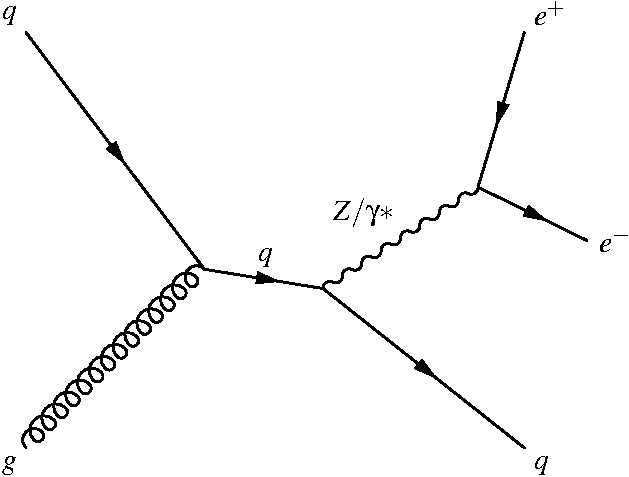
\includegraphics[width=\linewidth]{figures/feyn_qg_to_q_to_zq.pdf}
        \caption{}
        \label{fig:feyn_qg_to_q_to_zq}
    \end{subfigure}
    \caption[
        Higher order in \alphastrong \Ztoee Feynman diagrams.
    ]{
        Higher order in \alphastrong \Ztoee Feynman diagrams.
        \Cref{fig:feyn_qqbar_to_zg,fig:feyn_qbarq_to_zg} are ISR where one of
        the incoming quarks radiates a gluon. In
        \cref{fig:feyn_qg_to_zq,fig:feyn_qg_to_q_to_zq} the quark radiates a
        \Z.
    }
    \label{fig:higher_order_z_diagrams}
\end{figure}
